\subsection{Funktionsweise des Clients}
\label{sec:funktionsweise}


Der Client selber arbeitet folgendermaßen:

Beim Start wird die Konfiguration aus der  Datei config.cfg eingelesen, wenn diese nicht gefunden
wird, nutzt der Client die fest eingestellten Standardwerte. Die config.cfg
hat folgende Struktur:

\begin{lstlisting}[language={},captionpos=b,caption={Aufbau der config.cfg},label={aufbau_config}]
#Kommentarzeile (wird ignoriert)
Sonaranzahl als int
#Kommentarzeile (wird ignoriert)
COM-Port, an dem der Roboter angeschlossen ist, als String
#Kommentarzeile (wird ignoriert)
Schrittweite fuer die Anlerndrehungen als int in Grad
#Kommentarzeile (wird ignoriert)
Anzahl der 360Grad Drehungen als int
#Kommentarzeile (wird ignoriert)
Server-IP als String
#Kommentarzeile (wird ignoriert)
Pixel in der Karte pro mm als double
\end{lstlisting}

Ein Beispielkonfiguration für den Fahrstuhlvorraum vor dem
Robotik-Labor im Braunschweiger Informatik\-zentrum wäre z. B.
\begin{lstlisting}[language={},captionpos=b,caption={Ein Beispiel für eine komplette config.cfg},label={beispiel_config}]
#Anz Sensoren
8
#COM Port
COM5
#Schrittweite fuer die Anlerndrehungen
15
#Anzahl der 360Grad Drehungen
1
#Server-IP
134.169.36.241
#Pixel pro mm
0.05081
\end{lstlisting}
Die Standardwerte sind (16, COM3, 45, 0, 127.0.0.1, 1).

Danach wird die Verbindung zum Roboter hergestellt und der Partikelfilter
mit 10000 Partikeln initialisiert und das erste Mal gefiltert. Danach
erfolgt die konfigurierte Anzahl an Drehungen in der konfigurierten
Schrittweite um die erste Positionierung zu verbessern. Nach jedem
Drehschritt wird einmal gefiltert. Nach den Drehungen wird noch einmal
gefiltert und der Rückgabewert als Startposition genommen. Erst jetzt wird
die Verbindung zum Server hergestellt und die Roboterposition übermittelt,
sowie ein Thread gestartet, der regelmäßig die Structs \lstinline|RobotInformation|,
\lstinline|PathInformation| und \lstinline|SearchInformation| mit dem
Server abgleicht.  Sie enthalten die zum Steuern des Clients, sowie zur
Durchführung der Suche notwendigen Informationen.  Nach
Verbindungsaufbau wartet der Client bis der Server die Suche startet. 
Sobald die Suche startet, wird ein  Thread zur
Ballerkennung gestartet und der Client geht in seine Fahrschleife über, die
 erst endet, wenn der Ball gefunden wurde oder stoppt, wenn der Server
 die Suche pausiert oder beendet. Solange die Fahrschleife aktiv ist,
 wartet der Client auf den nächsten anzufahrenden Punkt vom Server,
sobald er diesen erhalten hat fährt der Roboter den Punkt an.
\begin{nofloat}{figure}
  \centering
  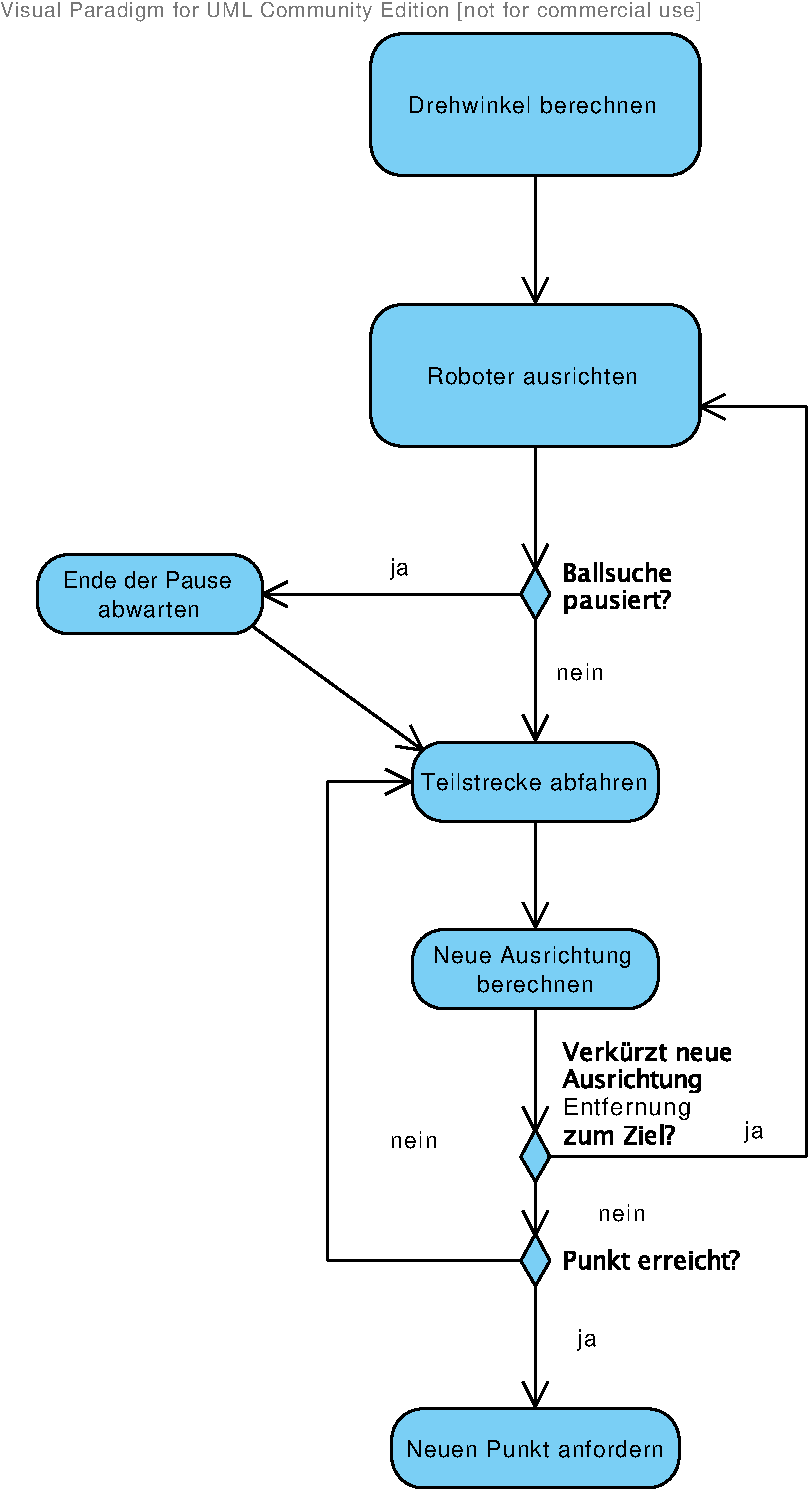
\includegraphics[width=0.45\linewidth]{bilder/fahrschleife_uml}
\caption{Ablauf der Fahrschleife des Clients}
\end{nofloat}
Dies geschieht schrittweise:\\
Zuerst wird die Richtung und der Drehwinkel der Drehung für eine
Ausrichtung zum Punkt berechnet. Dazu wird der Winkel zwischen dem
Ausrichtungsvektor des Roboters und dem Vektor vom Roboter zum Punkt berechnet und dann geprüft,
ob der Vektor zwischen Roboterposition und dem Punkt um den ermittelten
Winkel im Uhrzeigersinn oder gegen den Uhrzeigersinn von der
Roboterausrichtung aus liegt um die Drehrichtung zu ermitteln. Dann wird
der Roboter entprechend der ermittelten Werte zum Punkt hin gedreht.
Dann wird, falls die Suche gerade pausiert, gewartet bis der Server die
Pause beendet. Danach wird 
\lstinline|drivingTime * driveLengthWeight| ms gefahren, wobei drivingTime die
Fahrtzeit pro Schritt ist und driveLengthWeight ein Anpassungsfaktor der
Fahrzeit ist für den Fall, dass die Reststrecke in weniger als der
Fahrzeit pro Schritt zurückgelegt werden kann. Dazu wird aus den gefahrenen Strecken in jedem
Fahrtschritt und der jeweiligen Fahrtzeit die Geschwindigkeit in px pro ms
berechnet und über die Schritte der exponentiell geglättete Mittelwert
berechnet, woraus dann \lstinline|driveLengthWeight| für die Reststrecke berechnet wird
, wenn die zu klein für die normale Fahrzeit ist. 
Dann wird eine neue Ausrichtung zum Punkt berechnet und mit der aktuellen
 verglichen, verkürzt sich dadurch die Entfernung zum Ziel, wird der
Roboter neu ausgerichtet, ansonsten wird die alte Ausrichtung beibehalten.
Danach wird wieder eine Teilstrecke gefahren usw. bis sich dem Punkt auf
einen Abstand unterhalb einer Toleranzschwelle angenährt wurde
(\lstinline|delta_pos|). 
Die Toleranzschwelle ist nötig, da aufgrund der Ungenaugkeiten des
Sonar-Partikelfilters nicht immer eine genaues Erreichen der
Zielposition gewährleistet werden kann.  Auf die prinzipiellen
Ungenauigkeiten des Partikelfilters wird näher im Abschnitt
\ref{cha:evaluation} Evaluation
ab Seite \pageref{cha:evaluation} eingegangen. 
Danach wird gewartet, bis der Server das Erreichen des Punktes registriert
hat und ein neuer, anzufahrender Punkt übermittelt wurde.






%%% Local Variables: 
%%% mode: latex
%%% TeX-master: "template"
%%% End: 
